\documentclass[a4paper, 11pt]{article}
\usepackage{comment} % enables the use of multi-line comments (\ifx \fi) 
\usepackage{fullpage} % changes the margin
\usepackage[linesnumbered,ruled,french, onelanguage,vlined]{algorithm2e}
\RestyleAlgo{boxruled}
\usepackage{amsmath}
\usepackage[makeroom]{cancel}

\usepackage{graphicx}
\usepackage[]{textcomp}

\usepackage{geometry}
 \geometry{
 a4paper,
 left=15mm,
 right=15mm,
 top=15mm,
 }
 
\usepackage{pgfplots}
  \pgfplotsset{compat=newest}
  %% the following commands are needed for some matlab2tikz features
  \usetikzlibrary{plotmarks}
  \usetikzlibrary{arrows.meta}
  \usepgfplotslibrary{patchplots}
  \usepackage{grffile}
  
  \usepackage{tikz}
	\definecolor{mycolor1}{rgb}{0.00000,0.44700,0.74100}%
\definecolor{mycolor2}{rgb}{0.85000,0.32500,0.09800}%
\definecolor{mycolor3}{rgb}{0.92900,0.69400,0.12500}%

\SetKwIF{Si}{SinonSi}{}{Si}{}{Sinon}{}{Fin}

\SetKwFor{Pour}{Pour}{}{Fin}

\makeatletter
\def\blfootnote{\xdef\@thefnmark{}\@footnotetext}
\makeatother


\begin{document}

\noindent
\large\textbf{Mini-Projet C\raisebox{.5\height}{\scalebox{.5}{++}}} \hfill \textbf{RIBER Rafael} \\
\large\textbf{ColoReduce}\hfill \textbf{EL-BA1}\\
\normalsize ICC Pratique - CS-119\\
\hfill Novembre - Décembre 2018

\section*{Phase d'analyse}
Le programme est divisé en 5 fonctions de lecture regroupées sous la fonction \texttt{fileRead}, 4 fonctions de transformation (\texttt{normalize}, \texttt{filter}, \texttt{getPixelValue} et \texttt{blackEdge}), et 2 fonctions de rendu (\texttt{render} et \texttt{printRGB}):
\subparagraph{\underline{\textit{Lecture:}}}
Au sein de la fonction \texttt{fileRead}, executée dans \texttt{main}, on commence par déclarer une structure \texttt{"input"} de type \texttt{InputImg}. On execute ensuite les fonctions \texttt{inputReduced, inputThresholds, inputFilters, inputDimensions} et \texttt{inputPixels} qui remplissent chacune un champ de cette structure qui leur est passée par référence, respectivement le nombre \texttt{nbR} et les valeurs des couleurs réduites, les valeurs des seuils, le nombre de filtres \texttt{nbF}, les dimensions \texttt{nbL} et \texttt{nbC}, et les différentes couleurs des pixels de l'image à traiter, tout en vérifiant la validité de ces données et en renvoyant des erreurs en cas d'une mauvaise valeur. Le résultat de cette lecture est stocké dans la structure de type \texttt{InputImg} appelée \texttt{"image"} au sein de la fonction \texttt{main}. La fonction \texttt{colorRead}, qui lit 3 valeurs d'intensité et les stocke sous forme d'une structure \texttt{Color} est utilisée tout au long de la partie lecture pour lire les différentes valeurs RVB en entrée.

\subparagraph{\underline{\textit{Seuillage:}}}
Cette structure est ensuite passée par référence à la première fonction de transformation executée dans \texttt{main} appelée \texttt{normalize}, qui crée un tableau de type \texttt{NormImg} appelé \texttt{"normOut"}, calcule pour chaque pixel son intensité normalisée $I_N$ à partir des intensités RVB de ce dernier et détermine ensuite le code couleur de chaque pixel selon la valeur de cette intensité, ainsi que les seuils et la liste de couleurs réduites donnés en entrée. Le résultat de cette opération est stocké au sein de \texttt{main} dans un tableau \texttt{"norm"} de type \texttt{NormImg}.

\subparagraph{\underline{\textit{Filtrage:}}} On passe par référence à la fonction \texttt{filter} le tableau \texttt{"norm"}, ainsi que les dimensions de l'image d'entrée, le nombre \texttt{nbF}, et le nombre \texttt{nbR}. Pendant l'opération de filtrage (dans la fonction \texttt{filter}), la fonction \texttt{getPixelValue} calcule la nouvelle valeur de chaque pixel selon la valeur des pixels voisins. Le tableau est modifié par référence et l'image filtrée se trouve ainsi dans le tableau \texttt{"norm"} à la fin des \texttt{nbF} filtrages. La fonction \texttt{blackEdge}, executée au sein de \texttt{filter} après les filtrages, applique un bord noir d'un pixel de largeur tout autour de l'image filtrée, dans le cas où \texttt{nbF} $> 0$.

\subparagraph{\underline{\textit{Rendu et fin:}}} La fonction \texttt{render} génère un tableau \texttt{RGBImg} de structures de type \texttt{Color} contenant les valeurs RVB de chaque pixel à partir de l'indice entier calculé durant le seuillage et le filtrage ainsi que la couleur à l'indice correspondant dans la liste de couleurs réduites donnée en entrée. Le résultat est stocké dans le tableau \texttt{"rendered"} de type \texttt{RBGImg}.

La fonction \texttt{printRGB} affiche dans le terminal le tableau \texttt{rendered}, en ajoutant l'en-tête "P3" et en imprimant des espaces entre les valeurs RVB successives, ainsi que des retours à la ligne après chaque ligne de l'image.

\newpage
\section*{Algorithme de filtrage}
Ce pseudocode décrit un seul filtrage.\\
\begin{algorithm}[H]
\SetSideCommentLeft
    \KwIn{Tableau $source$ de taille $C \times L$, %nombre de filtres à appliquer $f$,
    nombre de couleurs réduites $r$.}
    \KwResult{Tableau $destination$\\
    \textbf{Remarque: }Les listes et tableaux sont indexés à 0.\\\hrulefill}
    
    %\underline{Filtrage}$(N,x,y,f,r)$\
    $destination \gets source$\\
    $val \gets 0$\\
    $count$ est une liste de longueur fixe $r$.
    
%    \Pour{$n$ \upshape{de} $1$ \upshape{à} $f$}
%      {
      	\Pour{$x$ \upshape{de} $1$ \upshape{à} $L - 1$}
      	  {
      	  \Pour{$y$ \upshape{de} $1$ \upshape{à} $C - 1$}
      	    {
    			$current \gets 0$\\
   				\Pour{$i$ \upshape{de} $-1$ \upshape{à} $1$}
   				  {
   				  	\Pour{$j$ \upshape{de} $-1$ \upshape{à} $1$}
   				  	  {
   				  	  	\Si{$i \neq 0$ \upshape{ou} $j \neq 0$}
   				  	  	  {
   				  	  	    $current \gets source$[$x + i$][$y + j$]\\
   				  	  	  	\Pour{$c$ \upshape{de} $0$ \upshape{à} $r$}
   				  	  	  	  {
   				  	  	  	  	\Si {$c = current$}
   				  	  	  	  		{
   				  	  	  	  			$count$[$c$] = $count$[$c$]$ + 1$\\
   				  	  	  	  			\Si {$count$\upshape{[$c$]} $\geq 6$}
   				  	  	  	  			  {
   				  	  	  	  			    $val \gets c$\\
   				  	  	  	  			    Continuer à la ligne 20.   
   				  	  	  	  			  }
   				  	  	  	  			\SinonSi{}{$val \gets 0$}
   				  	  	  	  		}
   				  	  	  	  }
   				  	  	  }
   				  	  }
   				  }
             $destination$[$x$][$y$] $\gets val$
      	    }
      	  }
%      	  $source \gets destination$
%        }
%        \Si{$f > 0$} 
%          {
%        	\Pour{$i$ \upshape{de} $0$ \upshape{à} $L$} 
%        	{
%        	  \Pour{$j$ \upshape{de} $0$ \upshape{à} $C$}
%        	  {
%                \Si{$i = 0$ \upshape{ou} $j = 0$ \upshape{ou} $i = L - 1$ \upshape{ou} $j = C - 1$}
%                  {
%                    $N$[$i$][$j$] $\gets 0$
%                  }
%              }
%            }
%        }
       \textbf{Sortir} $destination$
\caption{ \textsc{Filtrage}}
\end{algorithm}

\section*{Analyse de complexité}
\begin{minipage}{0.5\linewidth}
Dans le pire des cas, on parcourt tous les pixels n'étant pas en bordure de l'image $f$ fois, en parcourant une liste de courleurs de longueur maximale $r_{max}$ pour chacun des 8 voisins d'un pixel, puis les pixels de bordure une seule fois.

On a donc $N_i = (nbC - 2)(nbL-2)$ pixels à filtrer $f$ fois, et $N_b = (2nbC + 2(nbL-2))$ pixels en bordure, le tout multiplié par le nombre maximum de couleurs réduites $r_{max} = 255$ que l'on parcourt 8 fois pour les pixels voisins, ce qui donne:
\begin{align}
N_{pixels} &= 8 \cdot r_{max} \cdot (f \cdot N_i + N_b ) \nonumber \\
&= 8 \cdot r_{max}  (f \cdot (nbC - 2)(nbL-2) + (2nbC + 2(nbL-2))) \nonumber
\end{align}
On remarque que : $N_{pixels} \leq 8\cdot r_{max}\cdot f\cdot nbC\cdot nbL$\\

Et on a ainsi une complexité $\mathcal{O}(8\cdot r_{max}\cdot f\cdot nbC\cdot nbL)$.
\end{minipage}\hfil
\begin{minipage}{0.4\linewidth}
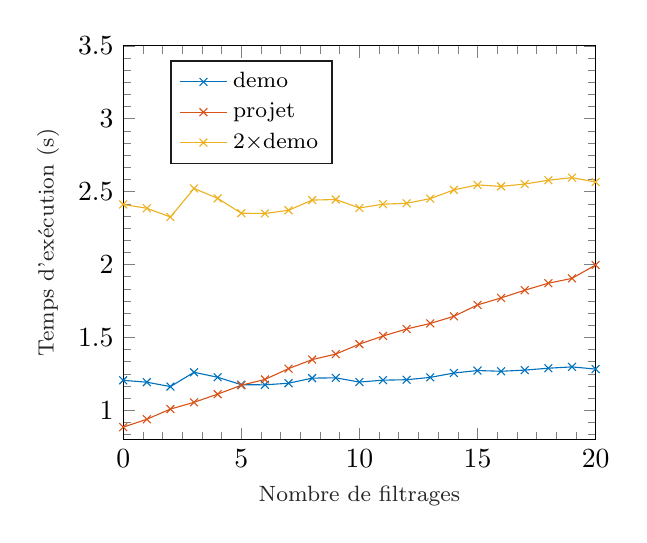
\begin{tikzpicture}
\begin{axis}[%
minor x tick num=5,
minor y tick num=5,
width=6cm,
height=5.0cm,
at={(2.087in,1.273in)},
scale only axis,
xmin=0,
xmax=20,
xminorticks=true,
xlabel style={font=\footnotesize\color{white!15!black}},
xlabel={Nombre de filtrages},
ymin=0.8,
ymax=3.5,
yminorticks=true,
ylabel style={font=\footnotesize\color{white!15!black}},
ylabel={Temps d'exécution (s)},
axis background/.style={fill=white},
legend style={font=\footnotesize,at={(0.1,0.7)}, anchor=south west, legend cell align=left, align=left, draw=white!11!black}
]
\addplot [color=mycolor1,mark=x]
  table[row sep=crcr]{%
0	1.206\\
1	1.193\\
2	1.163\\
3	1.261\\
4	1.227\\
5	1.176\\
6	1.175\\
7	1.186\\
8	1.221\\
9	1.223\\
10	1.194\\
11	1.207\\
12	1.21\\
13	1.226\\
14	1.256\\
15	1.273\\
16	1.268\\
17	1.276\\
18	1.289\\
19	1.298\\
20	1.283\\
};
\addlegendentry{demo}

\addplot [color=mycolor2,mark=x]
  table[row sep=crcr]{%
0	0.885\\
1	0.939\\
2	1.0087\\
3	1.055\\
4	1.111\\
5	1.172\\
6	1.212\\
7	1.286\\
8	1.348\\
9	1.386\\
10	1.454\\
11	1.51\\
12	1.558\\
13	1.596\\
14	1.645\\
15	1.723\\
16	1.771\\
17	1.824\\
18	1.872\\
19	1.905\\
20	1.997\\
};
\addlegendentry{projet}

\addplot [color=mycolor3,mark=x]
  table[row sep=crcr]{%
0	2.412\\
1	2.386\\
2	2.326\\
3	2.522\\
4	2.454\\
5	2.352\\
6	2.35\\
7	2.372\\
8	2.442\\
9	2.446\\
10	2.388\\
11	2.414\\
12	2.42\\
13	2.452\\
14	2.512\\
15	2.546\\
16	2.536\\
17	2.552\\
18	2.578\\
19	2.596\\
20	2.566\\
};
\addlegendentry{$2 \times$demo}

\end{axis}
\end{tikzpicture}%

{\blfootnote{Sur ce graphique, on voit le temps d'exécution de mon programme \texttt{projet} sur le fichier test \texttt{tree.txt} selon le nombre de filtrage appliqué, en comparaison avec le programme \texttt{demo}.}}

%\begin{tikzpicture}
%
%\begin{axis}[
%minor x tick num=5,
%width=6cm,
%height=6.0cm,
%at={(2.087in,1.268in)},
%scale only axis,
%xmin=0,
%xmax=20,
%xlabel style={font=\footnotesize\color{white!15!black}},
%xlabel={Nombre de filtrages},
%ymin=0,
%ymax=2.4,
%ytick={  0, 0.4, 0.8, 1.2, 1.6,   2, 2.4, 2.5},
%yminorticks=true,
%ylabel style={font=\footnotesize\color{white!15!black}},
%ylabel={Temps d'execution (s)},
%axis background/.style={fill=white},
%legend style={font=\footnotesize,at={(0.1,0.7)}, anchor=south west, legend cell align=left, align=left, draw=white!11!black}
%]
%\addplot [color=mycolor1]
%  table[row sep=crcr]{%
%0	1.211\\
%1	1.189\\
%2	1.182\\
%3	1.186\\
%4	1.174\\
%5	1.203\\
%6	1.206\\
%7	1.218\\
%8	1.219\\
%9	1.213\\
%10	1.323\\
%20	1.336\\
%30	1.452\\
%50	1.615\\
%100	2.125\\
%200	3.199\\
%500	6.334\\
%1000	11.453\\
%};
%\addlegendentry{Demo}
%
%\addplot [color=mycolor2]
%  table[row sep=crcr]{%
%0	0.857\\
%1	0.967\\
%2	1.011\\
%3	1.093\\
%4	1.125\\
%5	1.186\\
%6	1.219\\
%7	1.275\\
%8	1.346\\
%9	1.392\\
%10	1.458\\
%20	1.973\\
%30	2.542\\
%50	3.565\\
%100	6.248\\
%200	11.572\\
%500	27.524\\
%1000	54.477\\
%};
%\addlegendentry{Projet}
%
%\end{axis}
%\end{tikzpicture}%
\end{minipage}
\end{document}